\documentclass[a4paper, 16pt]{article}
\usepackage[utf8]{inputenc}
\usepackage[english, russian]{babel} 
\usepackage[left=20mm, top=20mm, right=20mm,
 bottom=20mm, head=1mm, foot=1mm]{geometry}
\usepackage{tikz} 
\usepackage{amsmath, amsfonts, amssymb}
\usepackage{graphicx}
\usepackage{fancybox, fancyhdr}
\usepackage{hyperref}
\usepackage{listings}
\usepackage{caption}
\usepackage{xcolor}
\pagestyle{fancy}
\fancyhf{}
\fancyhead[L]{Лабораторная работа №1}
\fancyhead[R]{Программирование промышленных контроллеров}
\fancyfoot[C]{\thepage}
\graphicspath{{images/}}
\usetikzlibrary{patterns}
\hypersetup{
    colorlinks=true,
    linkcolor=blue,
    filecolor=magenta,      
    urlcolor=cyan,
    pdftitle={contents setup},
    pdfpagemode=FullScreen,
}
\newcommand{\frc}[2]{\raisebox{2pt}{$#1$}\big/\raisebox{-3pt}{$#2$}}

\begin{document}
    \begin{titlepage}
        \begin{center}
        \vfill
        
        Федеральное государственное автономное образовательное учреждение высшего образования\\
        «Национальный Исследовательский Университет ИТМО»\ \\
        
        \vfill
        {\large\bf ЛАБОРАТОРНАЯ РАБОТА №1\\
            ПО ПРЕДМЕТУ <<ПРОГРАММИРОВАНИЕ ПРОМЫШЛЕННЫХ КОНТРОЛЛЕРОВ>>\
            ПО ТЕМЕ <<РАЗРАБОТКА ПРОГРАММЫ ДЛЯ ПЛК В СИСТЕМЕ CODESYS 3.5>>}
        \vfill
            
        \begin{flushright}  
            \begin{minipage}{.45\textwidth}
            {
                \hbox{Преподаватель: Крылова А. А.}
                \hbox{Выполнил: Румянцев А. А.}
                \hbox{Вариант: 1}
                \hbox{}
                \hbox{Факультет: СУиР}
                \hbox{Поток: ПРОГ. ПРОМ.ЛК 2.2}
            }
            \end{minipage}
        \end{flushright}
        
        \vfill
                
        Санкт-Петербург\\
        2024
        \end{center}
    \end{titlepage}
    \setlength{\parskip}{1.5mm}
    
    \tableofcontents

    \newpage
    \section{Задание}
    \noindent Автоматизация проветривания теплицы. В зависимости от изменения температуры в
    диапазоне от 25 до 35 градусов, плавно меняется состояние форточки. При 35 и
    более она должна быть полностью открыта


    \noindent
    \begin{align*}
        & \text{Вход:}\\
        & \text{– датчик температуры (значение в диапазоне от 15 до 40)}\\
        & \text{Выход:}\\
        & \text{– сервопривод (значение от 0 до 10). Где 10 это полное открытие форточки}
    \end{align*}


    \section{Структурная схема}
    \noindent На вход ПЛК подключается датчик температуры. Датчик передает показания в диапазоне от
    $15 \text{ до } 40^{\circ}$ цельсия. К выходу ПЛК подключается сервопривод, управляющий степенью
    открытия форточки в диапазоне от $0 \text{ до } 10$. Программа ПЛК работает совместно с визуализацией,
    которая эмулирует работу датчика и сервопривода


    \begin{figure}[!h]
        \centering
        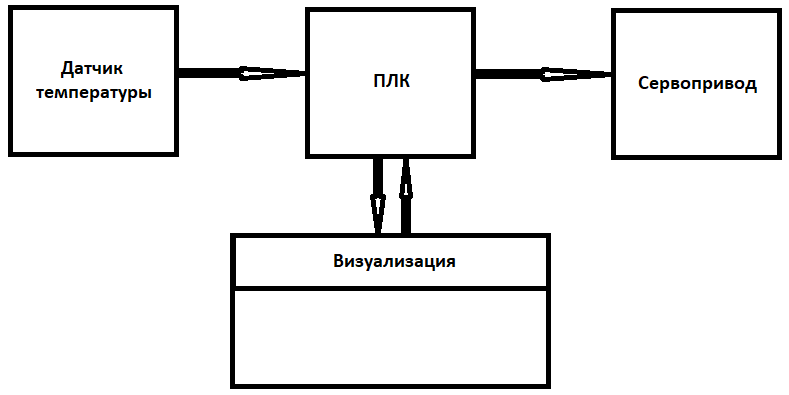
\includegraphics[scale=0.7]{scheme.png}
        \captionsetup{skip=0pt}
        \caption{Структурная схема}
        \label{Рис:1}
    \end{figure}


    \section{Дерево задач}
    \begin{figure}[!h]
        \centering
        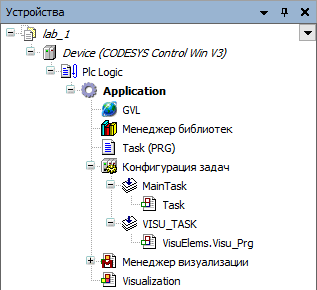
\includegraphics[scale=0.9]{tasks.png}
        \captionsetup{skip=0pt}
        \caption{Дерево задач}
        \label{Рис:2}
    \end{figure}


    \section{Список глобальных переменных}
    \noindent Переменная TEMPER\_{IN} отвечает за значение температуры с датчика температуры.
    Переменная\\OPEN\_{VAL} отвечает за подаваемые на сервопривод значения, которые будут регулировать открытие форточки\\
    \begin{figure}[!h]
        \centering
        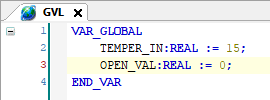
\includegraphics[scale=1]{gvl.png}
        \captionsetup{skip=0pt}
        \caption{Глобальные переменные}
        \label{Рис:3}
    \end{figure}


    \section{Код программы}
    \noindent В программе проверяются данные с датчика температуры. Если температура больше или равна 25 и
    меньше 35, то форточка плавно открывается пропорционально температуре по формуле ниже:
    $$
    \text{PROP} = \frac{\text{TEMPER\_IN} - \text{TEMPER\_MIN}}{\text{TEMPER\_MAX} - \text{TEMPER\_MIN}}
    $$
    $$
    \text{OPEN\_VAL}=\text{PROP } \cdot \text{ OPEN\_MAX}
    $$
    \noindent Если же температура меньше $25^{\circ}$, то на сервопривод подается минимальное
    значение открытости форточки. Если же больше $35^{\circ}$, то максимальное
    \begin{figure}[!h]
        \centering
        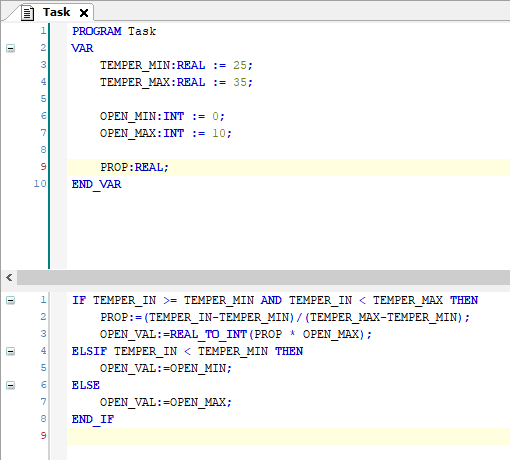
\includegraphics[scale=0.9]{prog.png}
        \captionsetup{skip=0pt}
        \caption{Программа}
        \label{Рис:4}
    \end{figure}


    \noindent В программе используется преобразование REAL\_{TO}\_{INT}, чтобы значение открытости
    форточки было целым числом


    \newpage
    \section{Визуализация}
    \begin{figure}[!h]
        \centering
        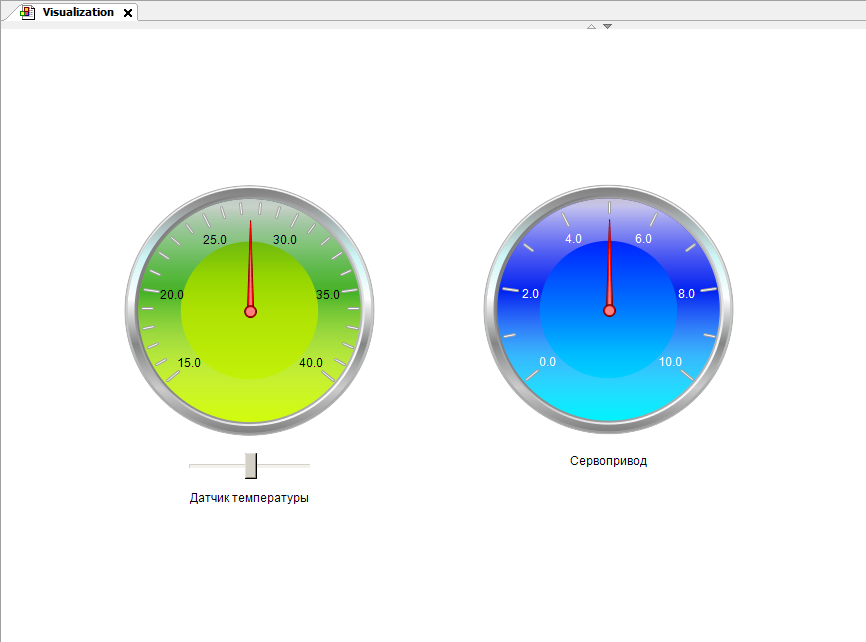
\includegraphics[scale=0.5]{visu.png}
        \captionsetup{skip=0pt}
        \caption{Визуализация}
        \label{Рис:5}
    \end{figure}
    \begin{figure}[!h]
        \centering
        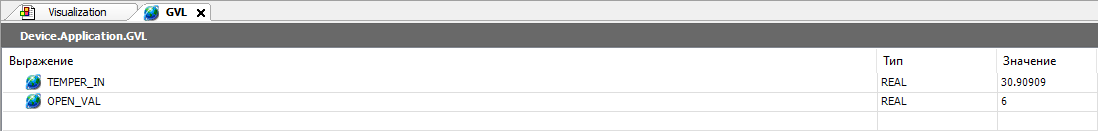
\includegraphics[scale=0.55]{visu2.png}
        \captionsetup{skip=0pt}
        \caption{Глобальные переменные при запуске}
        \label{Рис:6}
    \end{figure}


    \section{Демонстрация работы}
    \noindent Работу программы можно посмотреть на данном \href{https://drive.google.com/drive/folders/1dUwB7bgcupbfOugc56xTzlspjJ7I331R?usp=sharing}{гугл-диске}


    \section{Заключение}
    \noindent В ходе выполнения работы было разработано программное обеспечение для виртуального
    ПЛК Codesys Control Win V3 в системе Codesys 3.5. Программа написана на текстовом языке ST.
    В результате работы были освоены различные возможности в среде разработки программного обеспечения
    для ПЛК Codesys, а также изучен основной синтаксис языка ST
\end{document}